%%%% PROCESAR con PdfLaTeX !!!!!


\documentclass[12pt]{book}
\usepackage{geometry}\geometry{top=2cm,bottom=2cm,left=3cm,right=3cm}
\usepackage{amssymb}
\usepackage{amsmath}
\usepackage{graphicx}
\usepackage{txfonts}




\begin{document}
\thispagestyle{empty}

\begin {center}

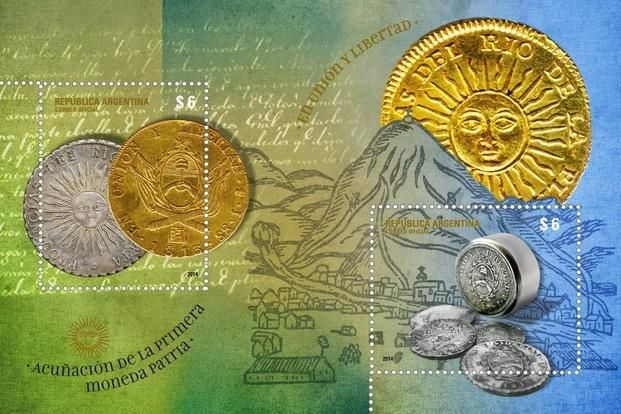
\includegraphics[scale=.4]{1484058646033.jpg}

\medskip
UNIVERSIDAD DE BUENOS AIRES

Facultad de Econom\'ia


\vspace{3cm}


\textbf{\large HISTORIA ECONOMICA SOCIAL GENERAL}

\vspace{2cm}


Este es un compendio de apuntes de clase, resumenes de la bibliograf\'ia obligatoria y es un aporte para los alumnos y los interesados en general.
De ninguna man\'era pretende ser una gu\'ia de estudio, ni remplaza las clases presenciales, el material oficial de la catedra esta disponible en el web site de la m\'ateria.
\\

\end {center}


\vspace{2.5cm}

\noindent Autor:\,	Isaac Edgar Camacho Ocampo
 
\noindent Carrera:\,	Licenciado en Econom\'ia

\vspace{1cm}

\vspace{1cm}

\noindent Buenos Aires, 2019

\newpage


\tableofcontents

\tableofcontents
\chapter{Revoluci\'on industrial}
\section{¿En que consistio la revolucion industrial?}
Capitulo 3,5 del libro de Barbero
 Comenzaremos con la siguiente interrogante ¿cual es el significado que los historiadores le atribuyen hoy al termino RI? Como vimos anteriormente no existe un consenzo entre los diferentes autores.
 \\
\\
\textbf{David landes propone 3 definiciones}
\begin{itemize}
 \item \textbf{revolucion industrial} en minuscula, se refiere al complejo de innovaciones tecnol\'ogicas que al sustituir la habilidad humana por maquinaria y la fuerza humana y animal por energ\'ia mec\'anica, provoca el paso desde un tipo de producci\'on artesanal a un tipo de producci\'on fabril naciendo as\'i la econom\'ia moderna.
 \item Otro significado que suele atribuirse al t\'ermino \textbf{Revoluci\'on Industrial}  es para referirse a cualquier proceso de cambio tecnol\'ogico r\'apido e importante.	En este sentido se habla tambien de una segunda y tercera revoluci\'on entendidas como una secuencia de innovaci\'on industrial historicamanete determinadas.
 \item \textbf{REVOLUCI\'ON INDUSTRIAL} con may\'uscula se refiere a la primera circunstancia hist\'orica de cambio desde una econom\'ia de base agraria y artesanal a otra dominada por la industria y la manufactura mecanizada, en este sentido la RI se inici\'o en inglaterra en el siglo XVIII y se expandio desde all\'i a los paises de la europa continental adem\'as de otras areas y transformo en menos de dos generaciones la vida del hombre occidental la naturaleza de su sociedad y sus relaciones con los demas pueblos.
 \end{itemize} 
\textbf{Por otro lado en historiador ingl\'es Peter Mathias} define la RI como (las fases iniciales del proceso de industrializaci\'on en el largo plazo), y señala dos criterios esenciales para definirla.
\begin{enumerate}
\item \textbf{La aceleraci\'on del crecimiento de la econom\'ia en su conjunto: }El crecimiento debe darse en un largo plazo y no responde al incrementos de los factores de producción sino Un aumento de la productividad que se traduzca en un incremento del producto per cápita .
\item \textbf{Cambios estructurales: }Incluyen entre otros la innovación tecnológica y organizativa la modernización institucional el desarrollo de un sistema de transporte y la movilización de la fuerza de trabajo este proceso genera a su vez modificaciones en la estructura de la economía en particular la reducción de la participación sectorial de la agricultura en el empleo y en el total de la producción
\end{enumerate}
Otro historiador inglés a \textbf{Wrigley} señala que la característica de la Revolución Industrial ha sido un aumento amplio y sostenido de los ingresos reales per cápita, sin un cambio de ese tipo el grueso del total de los ingresos si hubiese seguido gastando en alimentos y la fuerza de trabajo hubiese seguido siendo empleada en la Tierra.
\\
\\
Al aumentar la productividad del trabajo gracias a los procesos de innovación Se incrementa el producto por habitante En ese sentido wrigley contrapone dos modelos de crecimiento económico uno de ellos asociados a la economía orgánica avanzada y el otro a la economía basada en energía de origen mineral, el primero precede al segundo aunque existe una superposición 
\\
\\
En el modelo de economía orgánica avanzada la industria se abastecía esencialmente de materias primas animales y vegetales y el grueso de la energía se utilizaba era proporcionada por los hombres y los animales se suponía un límite muy preciso el crecimiento económico el uso de fuentes de energía de otro origen por ejemplo le permitió superar dichos límites incrementando de manera sostenida la productividad y las tasas de crecimiento de la economía.
\\
\\
Si combinamos estas definiciones podemos sostener que la Revolución Industrial consiste en un proceso de cambio estructural en el que se combinan tres elementos.
El rasgo más característico de dicho proceso es el nacimiento y el desarrollo de la industria fabril 

\begin{itemize}
\item \textbf{El crecimiento económico: }el crecimiento económico se debe principalmente al aumento de la productividad de la economía, (esto es producir mas con los mismos recursos) y dicho aumento de la productividad es posible gracias a la innovación tecnológica y organizativa.
\item \textbf{La innovación tecnológica y organizativa: }la principal Innovación organizativa consiste en el nacimiento del sistema de fábrica como alternativa a las formas de producción tradicional (la industria artesanal y la industria a domicilio) los rasgos esenciales de la innovación tecnológica son el uso de máquinas que reemplazan a la habilidad humana y la utilización de nuevas fuentes de energía inanimada que reemplazan a la fuerza humana y animal.
\item \textbf{Profundas transformaciones en la sociedad: }Por una parte se va produciendo un descenso de la participación de la agricultura en el total de la producción y de la proporción de mano de obra empleada en ese sector, al mismo tiempo se verifica un avance de la industria y los servicios que aumenta su participación en la producci\'on y el proceso de Urbanización a medida que avanza la industria fabril la población se van concentrando en ciudades, va creciendo el numero de ciudades, sus dimensiones y la proporción de población que pasa de la zona rural a la urbana
\end{itemize}

Al mismo tiempo aparece un nuevo tipo de sector social, Qué es la burguesía crece el número de empresarios qué invierten su capital en nuevas actividades y son propietarios de industrias una nueva burguesía Industrial buscando su lugar entre los sectores propietarios.
\\
\\
pero también en las clases bajas crecen ya que crecen junto con la expansión de los servicios y de las actividades administrativas como hemos señalado en las páginas precedentes la Revolución Industrial tuvo lugar no tuvo lugar en forma la mayor parte de los trabajos recientes han insistido en acentuar la complejidad del proceso de industrialización señalando que los cambios tuvieron lugar de una manera gradual y con fuertes diferencias regionales aún en Gran Bretaña en la primera nacional y a la difusión de la industria fue lenta y afectos de modo desigual a los diversos sectores pero el hecho de que haya tratado de un proceso gradual no invalida la existencia de una revolución industrial


\section{Tipos de insdustrias}

el nacimiento de la industria moderna Cuáles son los rasgos sobresalientes de la industria moderna Cómo se diferencia de las formas anteriores de producción industrial en su definición más general industria significa carácter transformación de la materia prima llevada a cabo por el hombre y existe como tal desde tiempos casi prehistóricos a lo largo de la historia se fueron sucediendo diferentes formas de producción industrial la primera fue la industria artesanal digámoslo así en nuestro del salón se caracterizaba por ser una forma de actividad en la que los productores o fabricantes utilizaban herramientas que requerían un alto nivel de habilidad la industria artesanal podía ser doméstica y se hacía se llevaba a cabo en la industria del productor o trabajador también existía la industria artesanal urbana que era una concentración como un pequeño taller en la que ha existido una organización jerárquica maestro-aprendiz oficial oficial en la que se llevan a cabo tareas la actividad urbana está fuertemente regulada por los gremios que establecían por ejemplo normas de calidad botas de producción ofrecen algunos rudimentarios beneficios sociales etcétera otra parte de nuestra era la industria a domicilio más o menos desde el siglo 16 fue desarrollándose paulatinamente una forma de producción industrial que tuvo una creciente expansión que recibía el nombre de Industria domicilio se caracteriza por ser un sistema descentralizado de producción en el que los trabajadores realizaban las tareas en sus domicilios herramientas en general les pertenecía trabajaban para un comerciante o empresario que se encargaba los quehaceres y le suministraba las materias primas alterando luego la producción los productos fabricados por estos en sus hogares pueden estar Ya listo para la venta en el Mercado o bien podrían requerir un proceso de terminación que era llevado a cabo en talleres urbanos el proceso de comercialización estaba en manos de los comerciantes empresarios y los productos se destinaban a mercados no locales propios o ultramarinos en este sistema de trabajo la mayor parte de los trabajadores eran campesinos que realizaron sus actividades en tiempos muertos en las que no estaban realizando tareas agrícolas la ventaja de esto era que la organización del trabajo consistía por un lado y es que era muy flexible es decir que la producción se reduce regulaba de acuerdo a la demanda y no existía una obligación por parte del empresario de mantener un vínculo permanente con los trabajadores es decir Los costos fijos serán mínimos y los salarios más bajos ya que no se aplicaban ningún tipo de regular de regulación que por ejemplo existía en las en la industria artesanal urbana los trabajadores aceptaron recibir un pago menor porque para ellos se trataba de una actividad complementaria ya que su ocupación principal era la agricultura la diferencia lindo urbana en la manufactura rural trabajaban también mujeres y niños cuyo apaga y la ínfima era menor en las zonas agrícolas menos fértiles Tuvo una característica muy importante que era que ofreció mejorar los ingresos de los campesinos el sistema de trabajo a domicilio sexenio fundamentalmente en la industria textil aunque también se utilizaban en otras ramas como la industria metalúrgica el vidrio los relojes
\chapter{Fundamentos teóricos}
\section{Teoría clásica}
\subsection{Definición de variables}
\subsection{Pruebas y refutaciones}
\section{Hipótesis}
\chapter{Resultados}
\section{Simulación de resultados}
\subsection{Suposiciones}
\subsection{Modelos}
\section{Resultados preliminares}
\section{Resultados postprocesados}
\subsection{Valores atípicos}
\subsection{Correlaciones}
\chapter{Conclusiones}
\end{document}
